\documentclass[crop,tikz,12pt]{standalone}

\usepackage{bbold}
\usepackage{tikz-qtree}
\usetikzlibrary{calc}
\usetikzlibrary{positioning}
\usetikzlibrary{shapes.misc}
\usetikzlibrary{arrows.meta}

% \definecolor{bg1}{RGB}{244,231,195}
% \definecolor{bg2}{RGB}{234,204,161}
\definecolor{bg1}{RGB}{186,212,148}
\definecolor{bg2}{RGB}{148,186,212}

\definecolor{bg1}{RGB}{203,233,107}
\definecolor{bg2}{RGB}{107,203,233}

% \definecolor{l1}{RGB}{209,148,106}

\makeatletter
\tikzset{font append/.style={font/.expand once=\tikz@textfont #1},
         font append/.value required}
\makeatother

\begin{document}

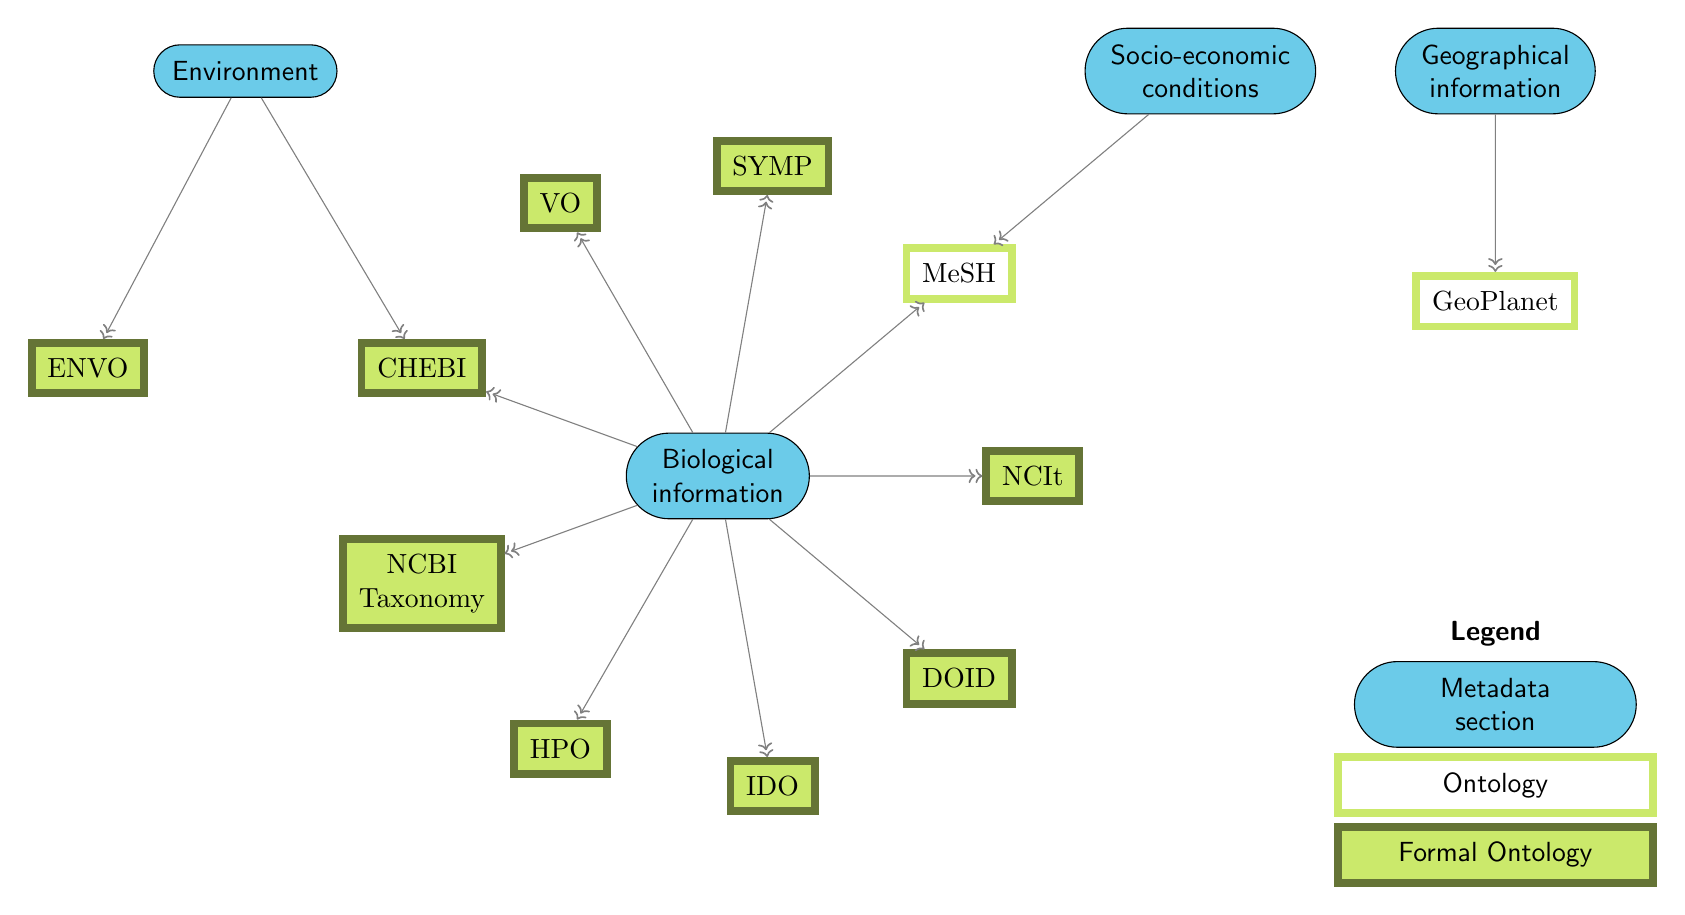
\begin{tikzpicture}[
    font=\sffamily,
    every node/.style={align=center},
    t/.style={
        fill=bg2,
        draw,
        rounded rectangle,
        inner sep=6pt
    },
    o/.style={
        draw=black!50!bg1,
        fill=bg1,
        line width=1mm,
        inner sep=2mm,
        font=\bbfamily
    },
    n/.style={
        o,
        fill=white,
        draw=bg1,
    },
    legend/.style={
        minimum width=4cm,
        font=\sffamily
    },
    l/.style={
        line width=0.4pt,
        color=black!50!white,
        -{Computer Modern Rightarrow[line width=0.6pt] . Computer Modern Rightarrow[line width=0.6pt]}
    },
]

\node [t] (bio) {Biological\\information};
\node [o] (ncit)     at ($(bio) + (0*40:4)$) {NCIt};
\node [n] (mesh)     at ($(bio) + (1*40:4)$) {MeSH};
\node [o] (symp)     at ($(bio) + (2*40:4)$) {SYMP};
\node [o] (vo)       at ($(bio) + (3*40:4)$) {VO};
\node [o] (chebi)    at ($(bio) + (4*40:4)$) {CHEBI};
\node [o] (taxonomy) at ($(bio) + (5*40:4)$) {NCBI\\Taxonomy};
\node [o] (hpo)      at ($(bio) + (6*40:4)$) {HPO};
\node [o] (ido)      at ($(bio) + (7*40:4)$) {IDO};
\node [o] (doid)     at ($(bio) + (8*40:4)$) {DOID};

\node [t] (soc) at ($(mesh) + (40:4)$) {Socio-economic\\conditions};

\node [t] (environment) at (-6, 42 |- soc) {Environment};
\node [o] (envo) at (-8, 42 |- chebi) {ENVO};

\node [t,right=of soc] (geo) {Geographical\\information};
\node [n,below=2 of geo] (geoplanet) {GeoPlanet};

\node [legend,font append=\bfseries] (legend) at (geo |- 9,-2) {Legend};
\node [t,legend,below=2pt of legend] (legend-meta) {Metadata\\section};
\node [n,legend,below=2pt of legend-meta] (legend-onto) {Ontology};
\node [o,legend,below=2pt of legend-onto] (legend-obo) {Formal Ontology};

\draw (bio) edge [l] (ncit);
\draw (bio) edge [l] (mesh);
\draw (bio) edge [l] (symp);
\draw (bio) edge [l] (vo);
\draw (bio) edge [l] (chebi);
\draw (bio) edge [l] (taxonomy);
\draw (bio) edge [l] (hpo);
\draw (bio) edge [l] (ido);
\draw (bio) edge [l] (doid);

\draw (environment) edge [l] (chebi);
\draw (environment) edge [l] (envo);

\draw (soc) edge [l] (mesh);

\draw (geo) edge [l] (geoplanet);

\end{tikzpicture}

\end{document}
